% !TEX program = xelatex
% Đồ án môn học Nhà kho dữ liệu và tích hợp
% Biên dịch: xelatex main.tex (chạy 2 lần để cập nhật mục lục)
\documentclass[13pt,a4paper]{extarticle}

\usepackage{fontspec}
\setmainfont{Times New Roman}
\usepackage[left=3cm,right=2cm,top=2.5cm,bottom=2.5cm]{geometry}
\usepackage{setspace,indentfirst,graphicx,float,xcolor,tikz}
\usepackage{array,tabularx,longtable,multirow,enumitem}
\usepackage{titlesec}
\usepackage[authoryear,round]{natbib}
\usepackage[font=it,labelsep=colon,justification=centering]{caption}
\usepackage[hidelinks,unicode]{hyperref}

% ---------- Thông tin báo cáo (sửa tại đây) ----------
\newcommand{\tenkhoa}{KHOA HỆ THỐNG THÔNG TIN}
\newcommand{\tennganh}{HỆ THỐNG THÔNG TIN QUẢN LÝ}
\newcommand{\tenchuyennganh}{KINH DOANH SỐ VÀ TRÍ TUỆ NHÂN TẠO}
\newcommand{\tendetai}{XÂY DỰNG GIẢI PHÁP KHO DỮ LIỆU TRÊN NỀN TẢNG MICROSOFT \mbox{FABRIC} CHO HOẠT ĐỘNG BÁN HÀNG CỦA ADVENTURE WORKS CYCLES}
\newcommand{\gvhd}{[Học hàm, học vị, họ tên GVHD]}
\newcommand{\svth}{[Họ tên sinh viên]}
\newcommand{\mssv}{[MSSV]}
\newcommand{\lop}{[Lớp]}
\newcommand{\thoigian}{TP.HCM, THÁNG ../....}
\newcommand{\coquan}{[Tên cơ quan kiến tập]}
\newcommand{\mentor}{[Họ tên người hướng dẫn tại cơ quan]}

% ---------- Trình bày chung ----------
\onehalfspacing
\setlength{\parindent}{1.27cm}
\setlength{\parskip}{6pt}
\graphicspath{{images/}}
\renewcommand{\contentsname}{MỤC LỤC}
\renewcommand{\listfigurename}{DANH MỤC HÌNH ẢNH}
\renewcommand{\listtablename}{DANH MỤC BẢNG BIỂU}
\renewcommand{\figurename}{Hình}
\renewcommand{\tablename}{Bảng}
\renewcommand{\refname}{TÀI LIỆU THAM KHẢO}
\counterwithin{figure}{section}
\counterwithin{table}{section}
\captionsetup[table]{position=top}

% ---------- Đề mục ----------
\setcounter{secnumdepth}{4}
\setcounter{tocdepth}{4}
\titleformat{\section}{\centering\bfseries}{}{0pt}{}
\titleformat{\subsection}{\bfseries}{\thesubsection}{0.5em}{}
\titleformat{\subsubsection}{\bfseries}{\thesubsubsection}{0.5em}{}
\titleformat{\paragraph}[hang]{\itshape}{\theparagraph}{0.5em}{}
\titlespacing*{\section}{0pt}{0pt}{12pt}
\titlespacing*{\subsection}{0pt}{12pt}{6pt}
\titlespacing*{\subsubsection}{0pt}{12pt}{6pt}
\titlespacing*{\paragraph}{0pt}{6pt}{6pt}

% \heading{...}: đề mục lớn không đánh số (LỜI CẢM ƠN, A., B., C., ...)
\newcommand{\heading}[1]{\clearpage\section*{#1}\addcontentsline{toc}{section}{#1}}
\newcommand{\chuong}[1]{\clearpage\refstepcounter{section}\section*{CHƯƠNG \thesection: #1}\addcontentsline{toc}{section}{CHƯƠNG \thesection: #1}}
% \phan{...}: "PHẦN n: ..." trong mục B; \phan[]{...} để không sang trang mới
\newcommand{\phan}[2][\clearpage]{#1\refstepcounter{section}%
  \section*{PHẦN \thesection: #2}\addcontentsline{toc}{phan}{PHẦN \thesection: #2}}
% Tiểu mục không đánh số, không vào mục lục
\newcommand{\tieumuc}[1]{\par\textbf{#1}\par}
\newcommand{\tieumucnghieng}[1]{\par\textit{#1}\par}

% ---------- Mục lục ----------
\makeatletter
\renewcommand*\l@section[2]{\addvspace{4pt}\@dottedtocline{1}{0em}{0em}{\bfseries #1}{\bfseries #2}}
\newcommand*\l@phan[2]{\@dottedtocline{1}{0.5cm}{0em}{\bfseries #1}{\bfseries #2}}
\renewcommand*\l@subsection[2]{\@dottedtocline{2}{1cm}{2em}{\bfseries #1}{\bfseries #2}}
\renewcommand*\l@subsubsection{\@dottedtocline{3}{1.5cm}{2.6em}}
\renewcommand*\l@paragraph{\@dottedtocline{4}{3cm}{3.4em}}
\newcommand*\toclevel@phan{1}
\makeatother

% ---------- Tiện ích giữ chỗ (xoá khi viết nội dung thật) ----------
\newcommand{\todo}[1]{\par{\color{gray}\textit{[#1]}}\par}
\newcommand{\nguon}[1]{\par\textit{Nguồn: #1}\par}
% \hinh{chú thích}{nhãn}: thay \fbox bằng \includegraphics
\newcommand{\hinh}[2]{\begin{figure}[H]\centering
  \fbox{\parbox[c][3.5cm][c]{0.7\textwidth}{\centering\color{gray}\textit{[Chèn hình]}}}
  \caption{#1}\label{#2}\end{figure}}
% \bang{chú thích}{nhãn}{số cột}{hàng tiêu đề}
\newcommand{\bang}[4]{\begin{table}[H]\centering\caption{#1}\label{#2}
  \begin{tabularx}{\textwidth}{|*{#3}{>{\centering\arraybackslash}X|}}\hline
  #4 \\ \hline
  \multicolumn{#3}{|c|}{\color{gray}\textit{[Nội dung bảng]}} \\ \hline
  \end{tabularx}\end{table}}
\newcommand{\dongcham}[1]{\par\noindent\foreach \i in {1,...,#1}{\makebox[\textwidth]{\dotfill}\\}\par\bigskip}

\begin{document}

% ================= BÌA =================
\begin{titlepage}
\begin{tikzpicture}[remember picture,overlay]
  \node[inner sep=0] at (current page.center)
    {
\includegraphics[width=\paperwidth,height=\paperheight]{cover-bg.jpg}};
  \node[font=\bfseries\fontsize{16}{20}\selectfont] at ([yshift=-45mm]current page.north) {\tenkhoa};
  \node[font=\bfseries,align=center] at ([yshift=-123mm]current page.north)
    {ĐỒ ÁN MÔN HỌC NHÀ KHO DỮ LIỆU VÀ TÍCH HỢP};
  \node[font=\bfseries,align=center,text width=16.5cm] at ([yshift=-164mm]current page.north) {\tendetai};
  \node[anchor=north west,align=left] at ([xshift=90mm,yshift=-194mm]current page.north west)
    {\textbf{GVHD:} \gvhd\\[4pt] \textbf{SVTH:} \svth\\[4pt] \textbf{MSSV:} \mssv};
  \node[font=\bfseries,text=white] at ([yshift=-271mm]current page.north) {\thoigian};
\end{tikzpicture}
\end{titlepage}
\setcounter{page}{1}

% ================= LỜI CẢM ƠN =================
\heading{LỜI CẢM ƠN}
\todo{Lời cảm ơn giảng viên hướng dẫn và những người hỗ trợ nhóm thực hiện đồ án.}

% ================= MỤC LỤC & CÁC DANH MỤC =================
\clearpage
\addcontentsline{toc}{section}{MỤC LỤC}
{\setlength{\parskip}{0pt}\tableofcontents}

\clearpage
\addcontentsline{toc}{section}{DANH MỤC HÌNH ẢNH}
{\setlength{\parskip}{0pt}\renewcommand{\numberline}[1]{Hình #1: }\listoffigures}

\clearpage
\addcontentsline{toc}{section}{DANH MỤC BẢNG BIỂU}
{\setlength{\parskip}{0pt}\renewcommand{\numberline}[1]{Bảng #1: }\listoftables}

\heading{DANH MỤC TỪ VIẾT TẮT}
{\singlespacing\renewcommand{\arraystretch}{1.5}
\begin{longtable}{|>{\centering\arraybackslash}p{2.2cm}|>{\centering\arraybackslash}p{6.1cm}|>{\centering\arraybackslash}p{6.1cm}|}\hline
\textbf{Từ viết tắt} & \textbf{Cụm từ đầy đủ} & \textbf{Diễn giải tiếng Việt} \\ \hline
\endhead
OLTP & Online Transaction Processing & Xử lý giao dịch trực tuyến \\ \hline
DW & Data Warehouse & Kho dữ liệu \\ \hline
BI & Business Intelligence & Trí tuệ kinh doanh \\ \hline
% ... bổ sung các từ viết tắt khác
\end{longtable}}

\heading{DANH MỤC THUẬT NGỮ}
{\singlespacing\renewcommand{\arraystretch}{1.5}
\begin{longtable}{|>{\centering\arraybackslash}p{1.5cm}|>{\centering\arraybackslash}p{6.2cm}|>{\centering\arraybackslash}p{6.9cm}|}\hline
\textbf{STT} & \textbf{Thuật ngữ gốc} & \textbf{Ý nghĩa} \\ \hline
\endhead
1 & Data Warehouse & Kho dữ liệu phục vụ phân tích \\ \hline
2 & Lakehouse & Nền tảng kết hợp lưu trữ hồ dữ liệu và khả năng quản lý bảng \\ \hline
3 & Star Schema & Mô hình hình sao gồm bảng sự kiện và các bảng chiều \\ \hline
% ... bổ sung các thuật ngữ khác
\end{longtable}}


\chuong{GIỚI THIỆU TỔNG QUAN}

\subsection{Bối cảnh thực tế}

Dữ liệu bán hàng được ghi nhận qua từng đơn hàng và dòng sản phẩm, còn người quản lý cần nhìn thấy doanh thu thay đổi ra sao theo thời gian, sản phẩm và khu vực. Để trả lời những câu hỏi đó, dữ liệu giao dịch phải được tổng hợp và đặt trong một cấu trúc có thể tra cứu theo nhiều góc nhìn.  Chaudhuri và Dayal~\citeyearpar{chaudhuri1997} cho thấy kho dữ liệu phục vụ phân tích cần dữ liệu lịch sử, được tích hợp và tổ chức phù hợp với các truy vấn tổng hợp.

Adventure Works Cycles là doanh nghiệp giả định trong một tình huống hướng dẫn của Microsoft. Trong tình huống này, dữ liệu giao dịch và thông tin ngoài giao dịch như hạn mức doanh số từ bảng tính đã được tập hợp vào kho dữ liệu quan hệ AdventureWorksDW2019. Microsoft mô tả các hạn chế ở tầng khai thác: báo cáo tĩnh khó cho phép đi sâu vào dữ liệu, người dùng mất thời gian tạo truy vấn do cấu trúc phức tạp và cách tính được viết riêng cho từng báo cáo có thể làm số liệu tổng hợp khác nhau. Tài liệu đánh giá kho dữ liệu này được thiết kế tốt và không có vấn đề lớn ở khâu nạp dữ liệu. Microsoft lựa chọn bổ sung Analysis Services để cải thiện truy vấn và tái sử dụng cách tính~\citep{microsoft-scenario}.

Tình huống hướng dẫn bắt đầu từ một kho dữ liệu đã có và tập trung khai thác dữ liệu bằng Analysis Services. Đồ án này sử dụng Adventure Works làm bối cảnh để thực hành thiết kế kho dữ liệu từ các bảng giao dịch của bộ dữ liệu. Công việc bao gồm xác định mức chi tiết của bảng sự kiện, thiết kế các chiều phân tích và thống nhất quy tắc tính chỉ tiêu, nhằm giải quyết hai hạn chế mà tình huống mẫu nêu ra là khó truy vấn theo nhiều góc nhìn và số liệu khác nhau giữa các báo cáo, trước khi kiểm tra kết quả trên báo cáo.

Microsoft Fabric được chọn làm nền tảng triển khai vì tài liệu tổng quan của Microsoft mô tả khả năng nạp, chuyển đổi, lưu trữ, phân tích và báo cáo trong cùng môi trường~\citep{microsoft-fabric}. Trong đó, mục Warehouse cho phép tổ chức dữ liệu theo cấu trúc phân tích; Microsoft~\citeyearpar{microsoft-warehouse} nêu mô hình hình sao và hình tuyết là các trường hợp phù hợp với Fabric Data Warehouse. Trên nền tảng này, đồ án xây dựng kho dữ liệu, quy trình cập nhật, báo cáo Power BI và mô hình dự báo doanh số.

\subsection{Lý do chọn đề tài}

Bài toán bán hàng của Adventure Works Cycles được chọn vì dữ liệu có thể liên kết giao dịch với sản phẩm, khách hàng, thời gian và khu vực. Các mối liên kết này cho phép thiết kế bảng sự kiện, bảng chiều và kiểm tra những chỉ tiêu cụ thể như doanh thu, số lượng bán và số đơn hàng. Nhờ vậy, số liệu trên báo cáo có thể được đối chiếu ngược với dữ liệu nguồn.

Để các chỉ tiêu được tính nhất quán, dữ liệu cần được chuẩn hóa trong một quy trình có thể chạy lại. Fabric cho phép triển khai quy trình đó cùng với kho dữ liệu và lớp báo cáo trong một môi trường. Dự báo doanh số cũng là yêu cầu của đồ án; chuỗi dữ liệu bán hàng đã xử lý trong kho sẽ là đầu vào để xây dựng và đánh giá mô hình dự báo.

Trong phạm vi đồ án môn học, mỗi quyết định thiết kế có thể được kiểm tra bằng kết quả cụ thể: dữ liệu sau xử lý có khớp nguồn hay không, các chỉ tiêu có cho cùng kết quả khi đối chiếu, và quy trình cập nhật có chạy ổn định. Những kết quả này cũng cho thấy các khâu cần điều chỉnh.

\subsection{Mục tiêu dự án}

\subsubsection{Mục tiêu tổng quan}

Mục tiêu tổng quan của dự án là xây dựng giải pháp kho dữ liệu trên nền tảng Microsoft Fabric phục vụ việc tích hợp, quản lý và khai thác dữ liệu bán hàng của Adventure Works Cycles. Giải pháp hướng đến việc tổ chức dữ liệu thành một hệ thống tập trung, nhất quán và thuận tiện cho phân tích đa chiều, từ đó hỗ trợ theo dõi tình hình kinh doanh, đánh giá hiệu quả bán hàng và nhận diện các xu hướng từ dữ liệu lịch sử.

Trên cơ sở kho dữ liệu được xây dựng, dự án kết hợp ứng dụng học máy, tự động hóa quy trình xử lý dữ liệu và trực quan hóa kết quả phân tích nhằm hỗ trợ ra quyết định trong hoạt động bán hàng. Đồng thời, thông qua quá trình triển khai, thử nghiệm và đánh giá, dự án làm rõ khả năng ứng dụng nền tảng Microsoft Fabric trong việc xây dựng một giải pháp dữ liệu xuyên suốt từ tích hợp dữ liệu nguồn đến khai thác thông tin phục vụ nhu cầu kinh doanh.

\subsubsection{Mục tiêu cụ thể}

Để đạt được mục tiêu tổng quan, dự án hướng đến các mục tiêu cụ thể sau:

Thứ nhất, khảo sát, mô tả và phân tích dữ liệu bán hàng của Adventure Works Cycles nhằm xác định cấu trúc dữ liệu, mối quan hệ giữa các bảng và các thông tin cần thiết cho bài toán phân tích. Đồng thời, đánh giá chất lượng dữ liệu, nhận diện các vấn đề về dữ liệu thiếu, trùng lặp hoặc không nhất quán để làm cơ sở xây dựng quy trình xử lý phù hợp.

Thứ hai, xây dựng quy trình tích hợp và xử lý dữ liệu trên nền tảng Microsoft Fabric, bao gồm thu thập, nạp, làm sạch, chuẩn hóa và chuyển đổi dữ liệu. Quy trình này hướng đến việc bảo đảm tính đầy đủ, nhất quán và toàn vẹn của dữ liệu trước khi đưa vào kho dữ liệu phục vụ phân tích và khai thác.

Thứ ba, thiết kế và triển khai kho dữ liệu theo mô hình đa chiều, tổ chức các bảng sự kiện và bảng chiều phù hợp với đặc điểm dữ liệu bán hàng. Kho dữ liệu cần đáp ứng nhu cầu phân tích các chỉ tiêu như doanh thu, số lượng sản phẩm bán ra và số lượng đơn hàng theo những chiều phân tích chủ yếu, bao gồm thời gian, sản phẩm, khách hàng và khu vực bán hàng.

Thứ tư, xây dựng và đánh giá mô hình học máy phục vụ hoạt động bán hàng trên cơ sở dữ liệu đã được xử lý và tổ chức trong kho dữ liệu. Nội dung này tập trung vào khai thác dữ liệu lịch sử để dự báo doanh số, phân tích xu hướng tiêu thụ và xem xét các yếu tố ảnh hưởng đến kết quả bán hàng, qua đó cung cấp thêm cơ sở cho việc lập kế hoạch kinh doanh.

Thứ năm, thiết lập cơ chế tự động hóa quy trình xử lý và cập nhật dữ liệu, bảo đảm các bước tích hợp, chuyển đổi và khai thác dữ liệu được thực hiện theo trình tự thống nhất. Đồng thời, theo dõi trạng thái thực thi và nhận diện lỗi phát sinh nhằm hỗ trợ duy trì hoạt động ổn định của hệ thống.

Thứ sáu, xây dựng các báo cáo và dashboard trực quan phục vụ theo dõi, phân tích và đánh giá tình hình bán hàng. Các báo cáo hướng đến việc thể hiện những chỉ tiêu kinh doanh chủ yếu, hỗ trợ so sánh kết quả giữa các thời kỳ, sản phẩm và khu vực, đồng thời trình bày kết quả dự báo để người sử dụng thuận tiện khai thác thông tin.

Thứ bảy, thử nghiệm và đánh giá giải pháp dựa trên các tiêu chí về chất lượng dữ liệu, tính chính xác của kết quả tổng hợp, hiệu quả truy vấn, khả năng vận hành quy trình tự động và mức độ đáp ứng của mô hình học máy. Trên cơ sở kết quả thực nghiệm, xác định những hạn chế của giải pháp và đề xuất hướng hoàn thiện, mở rộng trong tương lai.

\subsection{Đối tượng và phạm vi dự án}

\subsubsection{Đối tượng nghiên cứu}

Đối tượng nghiên cứu của dự án là dữ liệu bán hàng của Adventure Works Cycles và quy trình xây dựng giải pháp kho dữ liệu trên nền tảng Microsoft Fabric phục vụ khai thác dữ liệu này. Dự án tập trung vào các thông tin liên quan đến đơn hàng, chi tiết bán hàng, sản phẩm, khách hàng, thời gian và khu vực bán hàng, cùng với mối quan hệ giữa các đối tượng dữ liệu trong quá trình phân tích.

Dự án nghiên cứu mô hình tổ chức dữ liệu trong kho dữ liệu, quy trình tích hợp và chuyển đổi dữ liệu, phương pháp ứng dụng học máy cho bài toán bán hàng và cơ chế tự động hóa quá trình xử lý. Các báo cáo và dashboard được xây dựng hướng đến nhu cầu sử dụng của bộ phận quản lý và phân tích bán hàng, phục vụ theo dõi kết quả kinh doanh và tham khảo thông tin dự báo.

\subsubsection{Phạm vi nghiệp vụ bán hàng}
Dự án tập trung vào đơn hàng, chi tiết đơn hàng, sản phẩm, khách hàng và khu vực bán hàng. Các chỉ tiêu được xem xét gồm doanh thu, số lượng bán và số đơn hàng theo thời gian, sản phẩm, khách hàng và khu vực.

\subsubsection{Phạm vi dữ liệu}

Về phạm vi dữ liệu, dự án sử dụng dữ liệu Adventure Works được nhóm lựa chọn để triển khai, tập trung vào các bảng liên quan đến hoạt động bán hàng và những bảng nghiệp vụ cần thiết để bổ sung thông tin phân tích. Phạm vi thời gian được giới hạn trong khoảng dữ liệu lịch sử có sẵn của bộ dữ liệu sử dụng. Việc phân tích và đánh giá được thực hiện trên bộ dữ liệu này trong bối cảnh doanh nghiệp giả định.

\subsubsection{Phạm vi triển khai}

Về phạm vi xây dựng hệ thống, dự án triển khai quy trình thu thập, nạp, làm sạch, chuẩn hóa và chuyển đổi dữ liệu trên nền tảng Microsoft Fabric. Dữ liệu sau xử lý được tổ chức thành kho dữ liệu theo mô hình đa chiều, gồm các bảng sự kiện và bảng chiều phù hợp với yêu cầu phân tích bán hàng. Đồng thời, dự án thiết lập quy trình tự động hóa việc xử lý và cập nhật dữ liệu theo lịch hoặc kịch bản thử nghiệm.

Về phạm vi phân tích, dự án tập trung vào các chỉ tiêu chủ yếu như doanh thu, số lượng sản phẩm bán ra và số lượng đơn hàng. Các chỉ tiêu được khai thác theo thời gian, sản phẩm, khách hàng và khu vực bán hàng nhằm theo dõi xu hướng, so sánh kết quả và nhận diện những đặc điểm đáng chú ý trong dữ liệu. Kết quả phân tích được thể hiện thông qua các báo cáo và dashboard trực quan.

Về phạm vi học máy, dự án tập trung xây dựng mô hình dự báo doanh số dựa trên dữ liệu lịch sử. Việc lựa chọn phương pháp và mức độ tổng hợp dữ liệu được xác định phù hợp với đặc điểm của bộ dữ liệu và kết quả khảo sát ban đầu. Mô hình được huấn luyện, thử nghiệm và đánh giá nhằm xem xét khả năng cung cấp thông tin tham khảo cho hoạt động lập kế hoạch bán hàng.

Về phạm vi thử nghiệm và đánh giá, dự án kiểm tra chất lượng dữ liệu sau xử lý, tính chính xác của các chỉ tiêu tổng hợp, khả năng truy vấn và mức độ vận hành ổn định của quy trình tự động hóa. Đối với mô hình học máy, việc đánh giá được thực hiện trên dữ liệu kiểm tra theo trình tự thời gian để xem xét mức độ phù hợp của kết quả dự báo. Kết quả thử nghiệm là cơ sở xác định những hạn chế và đề xuất hướng phát triển của giải pháp.

Dự án được triển khai ở quy mô đồ án môn học, tập trung mô phỏng và đánh giá giải pháp trong môi trường thử nghiệm. Các nội dung như vận hành hệ thống ở quy mô doanh nghiệp, tích hợp dữ liệu giao dịch thời gian thực, tối ưu toàn bộ hoạt động sản xuất và quản lý chuỗi cung ứng nằm ngoài phạm vi triển khai của đồ án.

\subsection{Công nghệ và nền tảng sử dụng}
\subsubsection{Microsoft Fabric}
Microsoft Fabric cung cấp các thành phần tích hợp, lưu trữ, xử lý và trình bày dữ liệu trong cùng một môi trường~\citep{microsoft-fabric}. Đồ án sử dụng nền tảng này để tổ chức luồng từ dữ liệu giao dịch đến dữ liệu phục vụ phân tích.
\subsubsection{OneLake và Lakehouse}
OneLake là lớp lưu trữ dùng chung trong Fabric; Lakehouse là nơi nhóm dự kiến tổ chức dữ liệu qua các tầng xử lý trước khi nạp vào kho dữ liệu~\citep{microsoft-fabric}.
\subsubsection{Fabric Data Factory}
Fabric Data Factory được định hướng dùng để thu thập và điều phối các bước nạp, chuyển đổi dữ liệu. Cấu hình pipeline và lịch chạy sẽ được trình bày ở chương triển khai sau khi hoàn tất thử nghiệm~\citep{microsoft-fabric}.
\subsubsection{Fabric Data Warehouse}
Fabric Data Warehouse là lớp dữ liệu quan hệ phục vụ truy vấn phân tích. Mô hình dự kiến dùng bảng sự kiện bán hàng và các chiều thời gian, sản phẩm, khách hàng, khu vực~\citep{microsoft-warehouse}.
\subsubsection{Fabric Data Science}
Nhóm dự kiến dùng notebook trong Fabric để thử nghiệm dự báo từ dữ liệu lịch sử. Biến đầu vào, cách tách tập huấn luyện và kết quả đánh giá chỉ được xác định sau khi kiểm tra dữ liệu thực tế~\citep{microsoft-fabric}.
\subsubsection{Power BI và Web Application}
Power BI là lớp trình bày các chỉ tiêu bán hàng từ mô hình phân tích. Web Application nằm trong đề cương dự án; phạm vi và cách kết nối cần được xác nhận khi triển khai~\citep{microsoft-fabric}.

\chuong{MÔ TẢ VÀ PHÂN TÍCH DỮ LIỆU BÁN HÀNG}

\subsection{Tổng quan về Adventure Works Cycles}

Adventure Works Cycles là một doanh nghiệp hư cấu do Microsoft dựng nên làm bối cảnh cho bộ cơ sở dữ liệu mẫu AdventureWorks và các bài hướng dẫn về công cụ phân tích của hãng. Theo mô tả của Microsoft, đây là một công ty sản xuất đa quốc gia quy mô lớn, chế tạo và phân phối xe đạp khung kim loại lẫn vật liệu composite cho các thị trường thương mại ở Bắc Mỹ, châu Âu và châu Á \citep{microsoft-scenario}. Trụ sở đặt tại Bothell, bang Washington, nơi công ty sử dụng 500 lao động, và đi kèm là nhiều nhóm bán hàng khu vực phân bố khắp địa bàn kinh doanh \citep{microsoft-scenario}.

Ở khâu sản xuất, công ty từng mua lại một cơ sở nhỏ tại Mexico là Importadores Neptuno, chuyên làm các linh kiện quan trọng rồi chuyển về Bothell để lắp ráp thành phẩm. Sau một năm tài chính thuận lợi, ban lãnh đạo muốn mở rộng thị phần theo ba hướng: nhắm quảng cáo vào nhóm khách hàng tốt nhất, mở rộng khả năng tiếp cận sản phẩm qua một website bên ngoài, và giảm chi phí bán hàng bằng cách hạ chi phí sản xuất. Cả ba hướng đều cần phân tích doanh số theo khách hàng, kênh bán và sản phẩm. Đó cũng là lý do hoạt động bán hàng được chọn làm trọng tâm của đồ án này.

Adventure Works Cycles phù hợp với đề tài là do chính Microsoft đã mô tả một môi trường phân tích tương tự. Trong kịch bản của hãng, dữ liệu giao dịch từ cơ sở dữ liệu AdventureWorks2012 được kết hợp với các thông tin phi giao dịch như chỉ tiêu doanh số lấy từ bảng tính, rồi hợp nhất vào kho dữ liệu AdventureWorksDW2019. Nhóm phụ trách kho dữ liệu của công ty đánh giá kho này là cơ sở dữ liệu chiều được thiết kế tốt, có chiều dùng chung và khóa thay thế. Nhờ vậy, bộ dữ liệu vừa cho ta nguồn giao dịch để xử lý, vừa cho một mô hình chiều hoàn chỉnh để đối chiếu khi thiết kế kho trên Microsoft Fabric~\citep{microsoft-scenario}.

\subsection{Tổng quan hoạt động bán hàng}
\subsubsection{Quy trình bán hàng}
Trong dữ liệu nguồn, một đơn hàng gồm bản ghi đầu đơn tại \texttt{Sales.SalesOrderHeader} và các dòng hàng tại \texttt{Sales.SalesOrderDetail}. Đầu đơn lưu ngày đặt hàng, khách hàng, khu vực, kênh đặt hàng và trạng thái; dòng hàng lưu sản phẩm, số lượng, đơn giá và chiết khấu. Quan hệ này cho phép đi từ giao dịch phát sinh đến số đo doanh thu ở mức từng sản phẩm trong đơn~\citep{aw-samples}.
\subsubsection{Các đối tượng tham gia hoạt động bán hàng}
Các đối tượng chính trong phạm vi phân tích là đơn hàng, sản phẩm, khách hàng và lãnh thổ bán hàng. Dữ liệu sản phẩm nối tiếp tới phân nhóm và danh mục; khách hàng có thể gắn với cá nhân hoặc cửa hàng. Những quan hệ này được mô tả trong script nguồn \texttt{AdventureWorks/raw/instawdb.sql} và sơ đồ ở Hình~\ref{fig:aw-oltp-schema}.
\subsubsection{Các chỉ tiêu đánh giá hoạt động bán hàng}
Các chỉ tiêu dự kiến gồm doanh thu dòng hàng, số lượng sản phẩm bán và số đơn hàng. \texttt{LineTotal} của dòng hàng được định nghĩa từ đơn giá, tỷ lệ chiết khấu và số lượng; \texttt{TotalDue} ở đầu đơn gồm tạm tính, thuế và phí vận chuyển. Khi so sánh hai mức số đo phải nêu rõ có cộng thuế và phí vận chuyển hay không~\citep{aw-samples}.
\subsection{Nguồn gốc và cấu trúc dữ liệu}
\subsubsection{Nguồn dữ liệu Adventure Works}

Bộ AdventureWorks do Microsoft công bố ban đầu để minh họa cách thiết kế cơ sở dữ liệu trên SQL Server 2008. Trong đó, AdventureWorks là mẫu xử lý giao dịch trực tuyến (OLTP), còn AdventureWorksDW là mẫu kho dữ liệu. Về sau Microsoft tiếp tục phát hành phiên bản mới theo từng đời SQL Server, hiện trải từ 2008 R2 đến 2025, và chia thành ba biến thể: OLTP cho các khối lượng công việc giao dịch thông thường, DW cho kho dữ liệu, và LT là bản gọn nhẹ rút ra từ OLTP~\citep{aw-samples}.

Đồ án lấy bộ dữ liệu thô OLTP làm đại diện cho nguồn dữ liệu, với bộ script và tệp dữ liệu được lấy từ kho mã nguồn sql-server-samples của Microsoft trên GitHub. Nhóm có lựa chọn này xuất phát từ bản chất của dữ liệu OLTP, vì đây là dữ liệu phát sinh trực tiếp từ vận hành, chưa được mô hình hóa cho mục đích phân tích, đúng với dạng đầu vào mà một kho dữ liệu trong thực tế phải tiếp nhận. Từ nguồn này, dữ liệu sẽ lần lượt đi qua quy trình Medallion chuẩn trên Microsoft Fabric để hình thành mô hình phục vụ phân tích. Bộ script kho dữ liệu cùng kho mã nguồn được dùng làm mô hình tham chiếu khi thiết kế lớp đích. Biến thể LT không được sử dụng vì đây chỉ là bản rút gọn của OLTP.

\subsubsection{Cấu trúc dữ liệu nguồn}

Nguồn dữ liệu OLTP mô hình hóa hoạt động của AdventureWorks Cycles theo hướng ghi nhận giao dịch, với lược đồ chuẩn hóa ở mức cao. Ở dạng này, mỗi loại thông tin được tách thành bảng riêng và liên kết với nhau qua khóa, nhằm hạn chế dư thừa và giữ tính nhất quán khi dữ liệu liên tục được ghi và sửa.

Toàn bộ cơ sở dữ liệu được chia thành năm lược đồ. Cách chia này bám theo các bộ phận chính của một doanh nghiệp sản xuất, nên dữ liệu về cùng một đối tượng thường nằm rải rác ở nhiều lược đồ, mỗi lược đồ ứng với một mảng nghiệp vụ được mô tả trong bảng dưới đây:

\begin{table}[htbp]\centering
\caption{Các lược đồ nghiệp vụ trong AdventureWorks OLTP}
\label{tab:aw-schemas}
\begin{tabularx}{\textwidth}{|l|X|}\hline
\textbf{Lược đồ} & \textbf{Vai trò} \\ \hline
HumanResources & Thông tin nhân sự \\ \hline
Person & Thông tin cá nhân, liên hệ và địa chỉ \\ \hline
Production & Sản phẩm và hoạt động sản xuất \\ \hline
Purchasing & Mua hàng và nhà cung cấp \\ \hline
Sales & Bán hàng và khách hàng \\ \hline
\end{tabularx}
\end{table}

Ngoài năm lược đồ trên còn có một số bảng hệ thống dùng để ghi nhận lỗi và lịch sử thay đổi cấu trúc cơ sở dữ liệu. Các bảng này nằm ở lược đồ dbo và không mang thông tin nghiệp vụ, nên nằm ngoài phạm vi khai thác của đồ án.

\begin{figure}[H]\centering
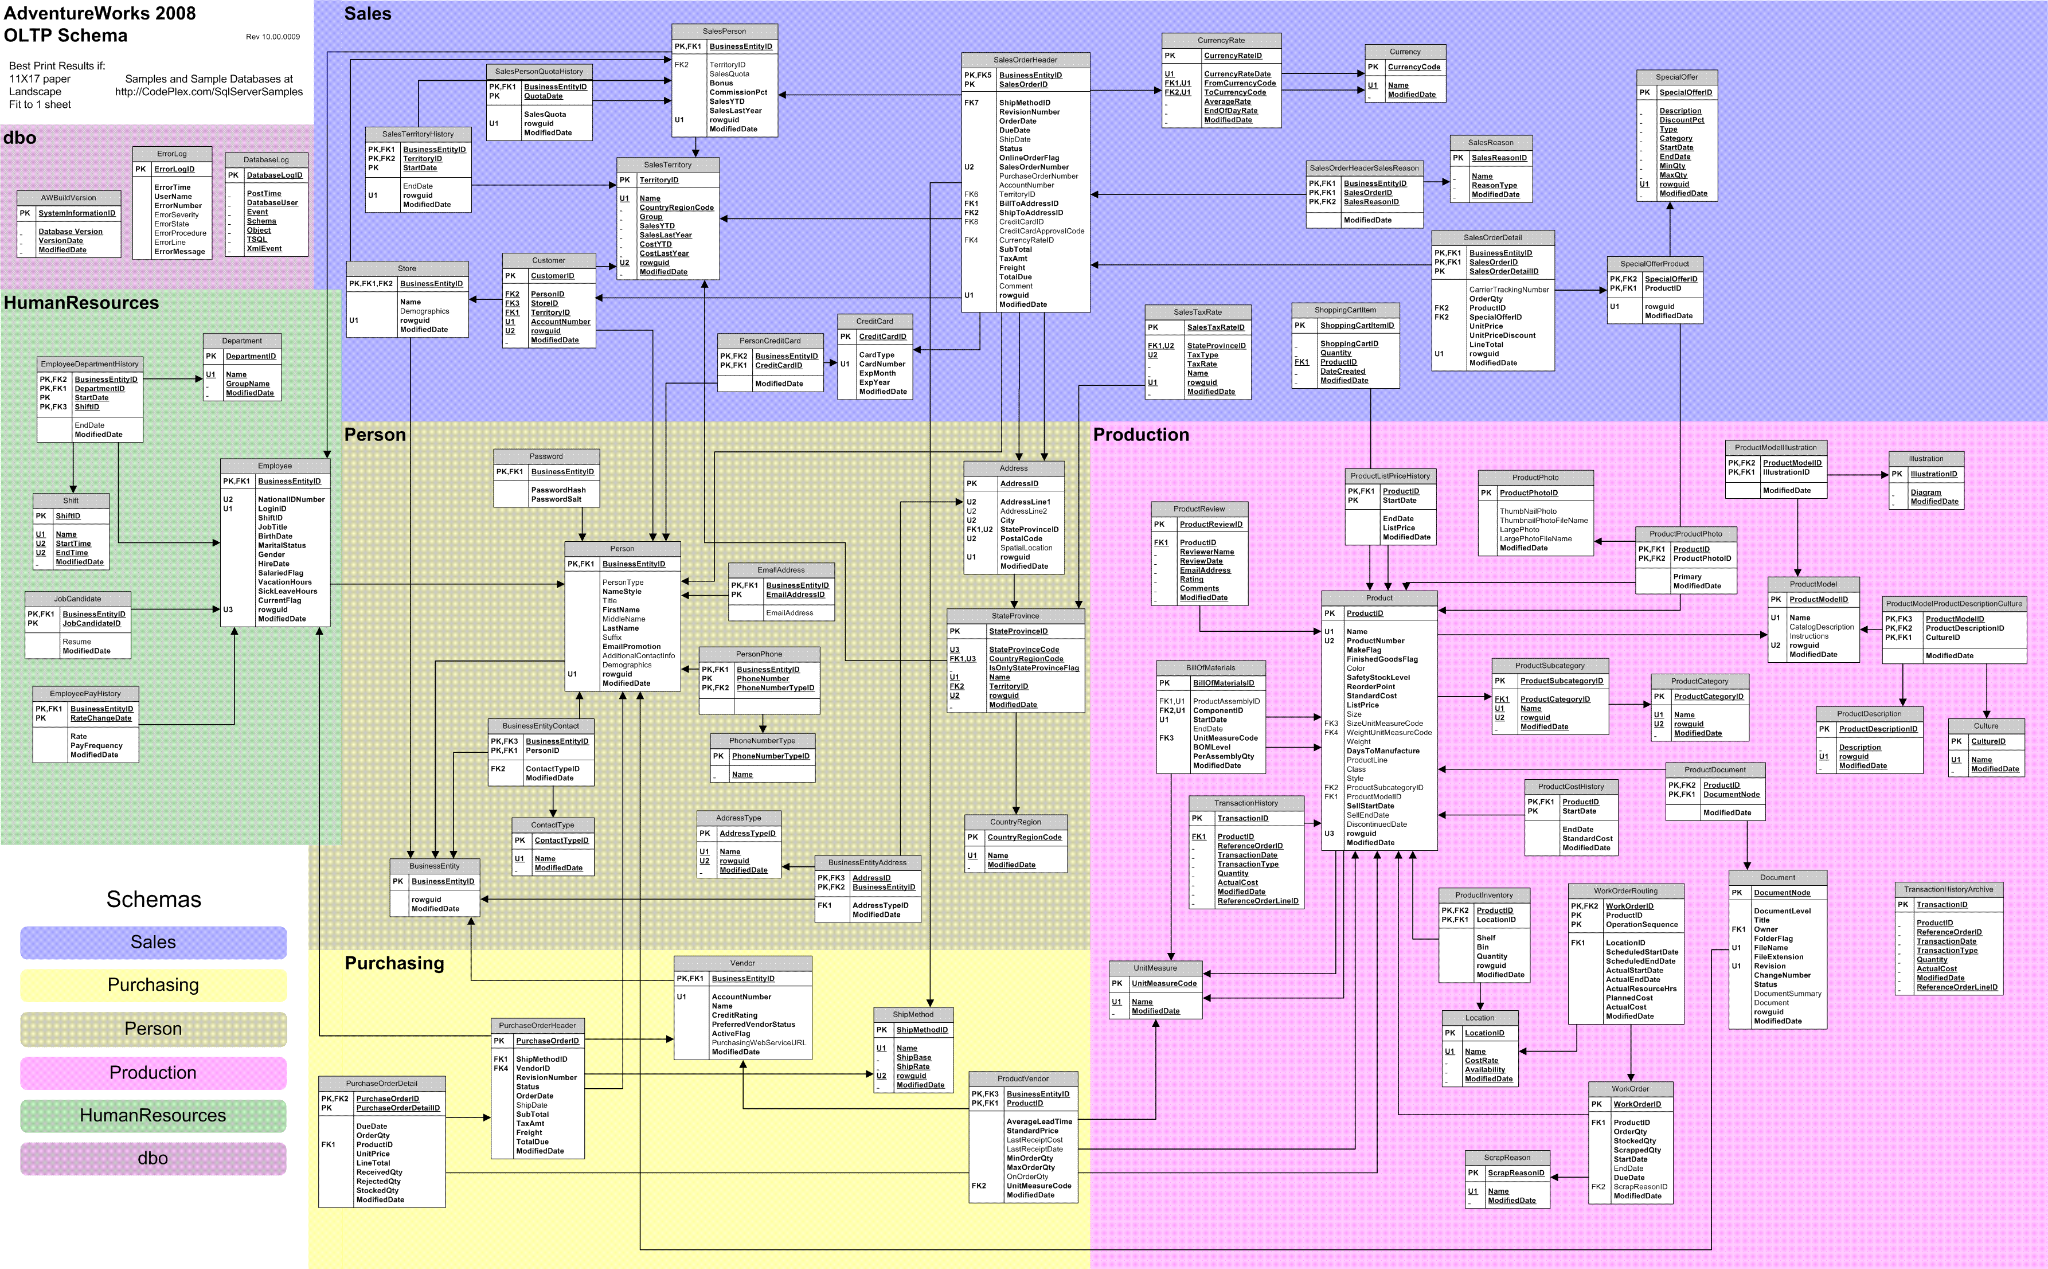
\includegraphics[width=\textwidth,height=0.6\textheight,keepaspectratio]{chapter-2/adventureworks-oltp-schema.png}
\caption{Sơ đồ tổng quát AdventureWorks OLTP 2008 (nguồn: \citealp{aw-schema}).}
\label{fig:aw-oltp-schema}
\end{figure}

Khác với OLTP, AdventureWorksDW được tổ chức theo mô hình chiều và gồm hai nhóm bảng. Nhóm thứ nhất là bảng sự kiện, có tiền tố Fact, chứa các số đo định lượng phát sinh từ nghiệp vụ. Nhóm thứ hai là bảng chiều, có tiền tố Dim, chứa các thông tin mô tả ngữ cảnh như khách hàng, sản phẩm, thời gian hay lãnh thổ. Các bảng liên kết với nhau bằng khóa thay thế có hậu tố Key, thay vì dùng trực tiếp mã nghiệp vụ của hệ thống nguồn.

Sự khác biệt giữa hai cách tổ chức này chính là lý do đồ án cần một quy trình chuyển đổi. OLTP được tối ưu cho việc ghi nhận giao dịch, còn mô hình chiều được tối ưu cho truy vấn và phân tích. Việc đưa dữ liệu từ nguồn thô đến mô hình chiều là nội dung của các chương sau.

\subsubsection{Các bảng dữ liệu phục vụ hoạt động bán hàng}
Nhóm bảng lõi gồm \texttt{SalesOrderHeader}, \texttt{SalesOrderDetail}, \texttt{Customer}, \texttt{SalesTerritory}, \texttt{Product}, \texttt{ProductSubcategory} và \texttt{ProductCategory}. Các bảng \texttt{Person} và \texttt{Store} bổ sung thông tin mô tả khách hàng. Khi triển khai cần kiểm tra khả năng nối từng bảng và cách xử lý khóa ngoại thiếu giá trị trước khi dùng làm chiều phân tích. Cấu trúc cột được đối chiếu từ \texttt{AdventureWorks/raw/instawdb.sql}~\citep{aw-samples}.
\subsubsection{Mối quan hệ giữa các bảng dữ liệu}
\texttt{SalesOrderDetail.SalesOrderID} nối với \texttt{SalesOrderHeader.SalesOrderID}; \texttt{ProductID} nối dòng hàng với sản phẩm. \texttt{CustomerID} và \texttt{TerritoryID} ở đầu đơn dẫn đến khách hàng và lãnh thổ. Từ sản phẩm có thể đi qua \texttt{ProductSubcategoryID} rồi \texttt{ProductCategoryID} để phân tích theo nhóm. Đây là đường nối dự kiến cho mô hình phân tích; số bản ghi mất liên kết cần được kiểm tra trên dữ liệu đã nạp.
\subsection{Khám phá và trực quan hóa dữ liệu}
\subsubsection{Phân tích doanh thu theo kênh bán hàng}
Cột \texttt{OnlineOrderFlag} ở đầu đơn có thể dùng để tách đơn đặt trực tuyến và đơn qua kênh khác. Bảng tổng hợp cần dùng cùng quy tắc trạng thái đơn và cùng định nghĩa doanh thu cho cả hai kênh.
\subsubsection{Phân tích doanh thu theo nhóm sản phẩm}
\texttt{ProductSubcategory} và \texttt{ProductCategory} cung cấp hai cấp phân nhóm. Khi tổng hợp, cần giữ cả sản phẩm chưa có phân nhóm để không làm mất doanh thu.
\subsubsection{Phân tích doanh thu theo thời gian}
\texttt{OrderDate} là mốc đặt hàng; \texttt{ShipDate} là mốc giao hàng và có thể trống. Nhóm sẽ chọn một ngày nghiệp vụ thống nhất trước khi tính chuỗi doanh thu theo tháng và năm.
\subsubsection{Phân tích khách hàng}
\texttt{CustomerID} cho phép đếm khách hàng phát sinh đơn. Việc phân loại cá nhân và cửa hàng dựa vào \texttt{PersonID} và \texttt{StoreID}; các trường hợp hai khóa cùng có giá trị cần được đối chiếu với định nghĩa trong dữ liệu nguồn.
\subsubsection{Phân tích doanh thu theo khu vực}
\texttt{TerritoryID} trên đầu đơn nối với \texttt{SalesTerritory}, nơi có tên lãnh thổ, quốc gia và nhóm khu vực. Doanh thu theo khu vực sẽ dùng lãnh thổ ghi tại thời điểm đơn hàng, tránh suy ngược từ địa chỉ hiện tại của khách hàng.
\subsection{Xác định yêu cầu dữ liệu cho giải pháp}
\subsubsection{Xác định quy trình nghiệp vụ}
Quy trình được chọn là bán hàng. Dữ liệu đầu đơn và dòng hàng là cơ sở để theo dõi doanh thu, số lượng bán và số đơn hàng theo các chiều phân tích.
\subsubsection{Xác định mức độ chi tiết dữ liệu}
Bảng sự kiện bán hàng dự kiến có một dòng cho mỗi \texttt{SalesOrderDetailID}. Mức chi tiết này giữ được liên hệ với sản phẩm, số lượng, giá và chiết khấu của từng dòng; các thuộc tính đầu đơn được đưa vào qua \texttt{SalesOrderID}.
\subsubsection{Xác định các chiều phân tích}
Những chiều tối thiểu gồm ngày đặt hàng, sản phẩm, khách hàng, lãnh thổ và kênh bán.
\subsubsection{Xác định các chỉ tiêu đo lường}
Các số đo tối thiểu gồm số lượng, doanh thu dòng hàng và số đơn hàng phân biệt. Thuế và phí vận chuyển ở mức đầu đơn sẽ được trình bày riêng để tránh cộng lặp khi một đơn có nhiều dòng.
\subsubsection{Xác định yêu cầu dữ liệu cho Machine Learning}
Bài toán dự báo doanh số cần chuỗi thời gian được tổng hợp ở một mức hạt và đơn vị tiền thống nhất. Tập huấn luyện và kiểm tra sẽ được tách theo thời gian; kết quả dự báo phải ghi rõ kỳ dự báo, dữ liệu lịch sử và sai số đánh giá trước khi đưa vào báo cáo.

% Chương 3–7: chỉ xuất hiện trong mục lục, không tạo trang nội dung.
\addtocontents{toc}{\protect\contentsline{section}{CHƯƠNG 3: XÂY DỰNG KHO DỮ LIỆU TRÊN MICROSOFT FABRIC}{--}{}}
\addtocontents{toc}{\protect\contentsline{subsection}{\protect\numberline{3.1}Kiến trúc tổng thể của giải pháp}{--}{}}
\addtocontents{toc}{\protect\contentsline{subsubsection}{\protect\numberline{3.1.1}Kiến trúc Microsoft Fabric}{--}{}}
\addtocontents{toc}{\protect\contentsline{subsubsection}{\protect\numberline{3.1.2}Luồng dữ liệu trong hệ thống}{--}{}}
\addtocontents{toc}{\protect\contentsline{subsubsection}{\protect\numberline{3.1.3}Vai trò của OneLake}{--}{}}
\addtocontents{toc}{\protect\contentsline{subsubsection}{\protect\numberline{3.1.4}Vai trò của Lakehouse và Data Warehouse}{--}{}}
\addtocontents{toc}{\protect\contentsline{subsection}{\protect\numberline{3.2}Tích hợp dữ liệu với Microsoft Fabric}{--}{}}
\addtocontents{toc}{\protect\contentsline{subsubsection}{\protect\numberline{3.2.1}Kết nối và thu thập dữ liệu nguồn}{--}{}}
\addtocontents{toc}{\protect\contentsline{subsubsection}{\protect\numberline{3.2.2}Xây dựng Data Pipeline}{--}{}}
\addtocontents{toc}{\protect\contentsline{subsubsection}{\protect\numberline{3.2.3}Xây dựng Dataflow Gen2}{--}{}}
\addtocontents{toc}{\protect\contentsline{subsubsection}{\protect\numberline{3.2.4}Tự động hóa quá trình tích hợp dữ liệu}{--}{}}
\addtocontents{toc}{\protect\contentsline{subsection}{\protect\numberline{3.3}Xây dựng Lakehouse theo Medallion Architecture}{--}{}}
\addtocontents{toc}{\protect\contentsline{subsubsection}{\protect\numberline{3.3.1}Tầng Bronze – dữ liệu nguồn}{--}{}}
\addtocontents{toc}{\protect\contentsline{subsubsection}{\protect\numberline{3.3.2}Tầng Silver – dữ liệu làm sạch và chuyển đổi}{--}{}}
\addtocontents{toc}{\protect\contentsline{subsubsection}{\protect\numberline{3.3.3}Tầng Gold – dữ liệu được chuẩn hóa phục vụ phân tích}{--}{}}
\addtocontents{toc}{\protect\contentsline{subsubsection}{\protect\numberline{3.3.4}Luồng chuyển đổi dữ liệu giữa các tầng}{--}{}}
\addtocontents{toc}{\protect\contentsline{subsection}{\protect\numberline{3.4}Thiết kế Data Warehouse cho hoạt động bán hàng}{--}{}}
\addtocontents{toc}{\protect\contentsline{subsubsection}{\protect\numberline{3.4.1}Xác định Business Process và Grain}{--}{}}
\addtocontents{toc}{\protect\contentsline{subsubsection}{\protect\numberline{3.4.2}Xây dựng Bus Matrix}{--}{}}
\addtocontents{toc}{\protect\contentsline{subsubsection}{\protect\numberline{3.4.3}Thiết kế Dimension Tables}{--}{}}
\addtocontents{toc}{\protect\contentsline{subsubsection}{\protect\numberline{3.4.4}Thiết kế Fact Tables}{--}{}}
\addtocontents{toc}{\protect\contentsline{subsubsection}{\protect\numberline{3.4.5}Xây dựng mô hình Star Schema}{--}{}}
\addtocontents{toc}{\protect\contentsline{subsection}{\protect\numberline{3.5}Xây dựng Fabric Data Warehouse}{--}{}}
\addtocontents{toc}{\protect\contentsline{subsubsection}{\protect\numberline{3.5.1}Tạo và cấu hình Data Warehouse}{--}{}}
\addtocontents{toc}{\protect\contentsline{subsubsection}{\protect\numberline{3.5.2}Xây dựng các bảng Dimension}{--}{}}
\addtocontents{toc}{\protect\contentsline{subsubsection}{\protect\numberline{3.5.3}Xây dựng các bảng Fact}{--}{}}
\addtocontents{toc}{\protect\contentsline{subsubsection}{\protect\numberline{3.5.4}Thiết lập khóa và mối quan hệ}{--}{}}
\addtocontents{toc}{\protect\contentsline{subsubsection}{\protect\numberline{3.5.5}Nạp và đồng bộ dữ liệu}{--}{}}
\addtocontents{toc}{\protect\contentsline{subsection}{\protect\numberline{3.6}Xây dựng Semantic Model}{--}{}}
\addtocontents{toc}{\protect\contentsline{subsubsection}{\protect\numberline{3.6.1}Thiết kế mô hình dữ liệu phân tích}{--}{}}
\addtocontents{toc}{\protect\contentsline{subsubsection}{\protect\numberline{3.6.2}Xây dựng Measures và KPI}{--}{}}
\addtocontents{toc}{\protect\contentsline{subsubsection}{\protect\numberline{3.6.3}Thiết lập Relationships và Hierarchies}{--}{}}
\addtocontents{toc}{\protect\contentsline{subsubsection}{\protect\numberline{3.6.4}Kết nối với Power BI}{--}{}}
\addtocontents{toc}{\protect\contentsline{section}{CHƯƠNG 4: XÂY DỰNG MÔ HÌNH HỌC MÁY CHO HOẠT ĐỘNG BÁN HÀNG}{--}{}}
\addtocontents{toc}{\protect\contentsline{subsection}{\protect\numberline{4.1}Chuẩn bị dữ liệu cho Machine Learning}{--}{}}
\addtocontents{toc}{\protect\contentsline{subsubsection}{\protect\numberline{4.1.1}Xác định bài toán dự báo}{--}{}}
\addtocontents{toc}{\protect\contentsline{subsubsection}{\protect\numberline{4.1.2}Xây dựng tập dữ liệu huấn luyện}{--}{}}
\addtocontents{toc}{\protect\contentsline{subsubsection}{\protect\numberline{4.1.3}Tiền xử lý và biến đổi dữ liệu}{--}{}}
\addtocontents{toc}{\protect\contentsline{subsection}{\protect\numberline{4.2}Xây dựng mô hình dự báo doanh số}{--}{}}
\addtocontents{toc}{\protect\contentsline{subsubsection}{\protect\numberline{4.2.1}Xác định biến và đặc trưng đầu vào}{--}{}}
\addtocontents{toc}{\protect\contentsline{subsubsection}{\protect\numberline{4.2.2}Huấn luyện mô hình}{--}{}}
\addtocontents{toc}{\protect\contentsline{subsubsection}{\protect\numberline{4.2.3}Tối ưu và lựa chọn mô hình}{--}{}}
\addtocontents{toc}{\protect\contentsline{subsubsection}{\protect\numberline{4.2.4}Đánh giá mô hình dự báo}{--}{}}
\addtocontents{toc}{\protect\contentsline{subsection}{\protect\numberline{4.3}Xây dựng mô hình dự báo nhu cầu và nguy cơ hết hàng}{--}{}}
\addtocontents{toc}{\protect\contentsline{subsubsection}{\protect\numberline{4.3.1}Xác định bài toán}{--}{}}
\addtocontents{toc}{\protect\contentsline{subsubsection}{\protect\numberline{4.3.2}Xây dựng tập dữ liệu huấn luyện}{--}{}}
\addtocontents{toc}{\protect\contentsline{subsubsection}{\protect\numberline{4.3.3}Huấn luyện mô hình}{--}{}}
\addtocontents{toc}{\protect\contentsline{subsubsection}{\protect\numberline{4.3.4}Đánh giá mô hình}{--}{}}
\addtocontents{toc}{\protect\contentsline{subsection}{\protect\numberline{4.4}Triển khai Machine Learning trên Microsoft Fabric}{--}{}}
\addtocontents{toc}{\protect\contentsline{subsubsection}{\protect\numberline{4.4.1}Fabric Data Science và Notebooks}{--}{}}
\addtocontents{toc}{\protect\contentsline{subsubsection}{\protect\numberline{4.4.2}Quản lý thí nghiệm và mô hình}{--}{}}
\addtocontents{toc}{\protect\contentsline{subsubsection}{\protect\numberline{4.4.3}Lưu trữ kết quả dự báo}{--}{}}
\addtocontents{toc}{\protect\contentsline{subsubsection}{\protect\numberline{4.4.4}Tích hợp kết quả dự báo vào Data Warehouse}{--}{}}
\addtocontents{toc}{\protect\contentsline{section}{CHƯƠNG 5: TỰ ĐỘNG HÓA VÀ KHAI THÁC DỮ LIỆU}{--}{}}
\addtocontents{toc}{\protect\contentsline{subsection}{\protect\numberline{5.1}Tự động hóa quy trình dữ liệu trên Microsoft Fabric}{--}{}}
\addtocontents{toc}{\protect\contentsline{subsubsection}{\protect\numberline{5.1.1}Cơ chế điều phối Data Pipeline}{--}{}}
\addtocontents{toc}{\protect\contentsline{subsubsection}{\protect\numberline{5.1.2}Lập lịch và kích hoạt quy trình}{--}{}}
\addtocontents{toc}{\protect\contentsline{subsubsection}{\protect\numberline{5.1.3}Tự động cập nhật dữ liệu}{--}{}}
\addtocontents{toc}{\protect\contentsline{subsubsection}{\protect\numberline{5.1.4}Tích hợp kết quả Machine Learning}{--}{}}
\addtocontents{toc}{\protect\contentsline{subsection}{\protect\numberline{5.2}Kiểm thử và đánh giá quy trình dữ liệu}{--}{}}
\addtocontents{toc}{\protect\contentsline{subsubsection}{\protect\numberline{5.2.1}Kiểm tra dữ liệu qua các tầng}{--}{}}
\addtocontents{toc}{\protect\contentsline{subsubsection}{\protect\numberline{5.2.2}Kiểm tra chất lượng dữ liệu tại tầng Silver}{--}{}}
\addtocontents{toc}{\protect\contentsline{subsubsection}{\protect\numberline{5.2.3}Kiểm tra tính đúng đắn của mô hình Data Warehouse}{--}{}}
\addtocontents{toc}{\protect\contentsline{subsubsection}{\protect\numberline{5.2.4}Kiểm tra dữ liệu đầu ra của Machine Learning}{--}{}}
\addtocontents{toc}{\protect\contentsline{subsection}{\protect\numberline{5.3}Khai thác dữ liệu với Power BI}{--}{}}
\addtocontents{toc}{\protect\contentsline{subsubsection}{\protect\numberline{5.3.1}Dashboard tổng quan hoạt động bán hàng}{--}{}}
\addtocontents{toc}{\protect\contentsline{subsubsection}{\protect\numberline{5.3.2}Dashboard phân tích khách hàng}{--}{}}
\addtocontents{toc}{\protect\contentsline{subsubsection}{\protect\numberline{5.3.3}Dashboard phân tích sản phẩm}{--}{}}
\addtocontents{toc}{\protect\contentsline{subsubsection}{\protect\numberline{5.3.4}Dashboard phân tích doanh thu}{--}{}}
\addtocontents{toc}{\protect\contentsline{subsubsection}{\protect\numberline{5.3.5}Dashboard phân tích khu vực và kênh bán hàng}{--}{}}
\addtocontents{toc}{\protect\contentsline{subsubsection}{\protect\numberline{5.3.6}Dashboard kết quả dự báo}{--}{}}
\addtocontents{toc}{\protect\contentsline{subsection}{\protect\numberline{5.4}Xây dựng và triển khai Web Application}{--}{}}
\addtocontents{toc}{\protect\contentsline{subsubsection}{\protect\numberline{5.4.1}Kiến trúc ứng dụng}{--}{}}
\addtocontents{toc}{\protect\contentsline{subsubsection}{\protect\numberline{5.4.2}Tích hợp dữ liệu từ Data Warehouse}{--}{}}
\addtocontents{toc}{\protect\contentsline{subsubsection}{\protect\numberline{5.4.3}Tích hợp kết quả Machine Learning}{--}{}}
\addtocontents{toc}{\protect\contentsline{subsubsection}{\protect\numberline{5.4.4}Triển khai ứng dụng}{--}{}}
\addtocontents{toc}{\protect\contentsline{section}{CHƯƠNG 6: THỬ NGHIỆM VÀ ĐÁNH GIÁ GIẢI PHÁP}{--}{}}
\addtocontents{toc}{\protect\contentsline{subsection}{\protect\numberline{6.1}Đánh giá Data Warehouse}{--}{}}
\addtocontents{toc}{\protect\contentsline{subsubsection}{\protect\numberline{6.1.1}Đánh giá tính đầy đủ và nhất quán của dữ liệu}{--}{}}
\addtocontents{toc}{\protect\contentsline{subsubsection}{\protect\numberline{6.1.2}Đánh giá mô hình Star Schema}{--}{}}
\addtocontents{toc}{\protect\contentsline{subsubsection}{\protect\numberline{6.1.3}Đánh giá khả năng truy vấn và khai thác dữ liệu}{--}{}}
\addtocontents{toc}{\protect\contentsline{subsection}{\protect\numberline{6.2}Đánh giá các mô hình Machine Learning}{--}{}}
\addtocontents{toc}{\protect\contentsline{subsubsection}{\protect\numberline{6.2.1}Đánh giá mô hình dự báo doanh số}{--}{}}
\addtocontents{toc}{\protect\contentsline{subsubsection}{\protect\numberline{6.2.2}Đánh giá mô hình dự báo nhu cầu và nguy cơ hết hàng}{--}{}}
\addtocontents{toc}{\protect\contentsline{subsection}{\protect\numberline{6.3}Đánh giá quy trình tự động hóa}{--}{}}
\addtocontents{toc}{\protect\contentsline{subsubsection}{\protect\numberline{6.3.1}Kết quả thực thi Data Pipeline}{--}{}}
\addtocontents{toc}{\protect\contentsline{subsubsection}{\protect\numberline{6.3.2}Kết quả cập nhật dữ liệu}{--}{}}
\addtocontents{toc}{\protect\contentsline{subsubsection}{\protect\numberline{6.3.3}Kết quả tích hợp Machine Learning}{--}{}}
\addtocontents{toc}{\protect\contentsline{subsection}{\protect\numberline{6.4}Đánh giá hệ thống báo cáo và Web Application}{--}{}}
\addtocontents{toc}{\protect\contentsline{subsubsection}{\protect\numberline{6.4.1}Kết quả Dashboard}{--}{}}
\addtocontents{toc}{\protect\contentsline{subsubsection}{\protect\numberline{6.4.2}Kết quả Web Application}{--}{}}
\addtocontents{toc}{\protect\contentsline{subsubsection}{\protect\numberline{6.4.3}Khả năng hỗ trợ hoạt động bán hàng}{--}{}}
\addtocontents{toc}{\protect\contentsline{subsection}{\protect\numberline{6.5}Đề xuất khai thác dữ liệu cho hoạt động bán hàng}{--}{}}
\addtocontents{toc}{\protect\contentsline{section}{CHƯƠNG 7: KẾT LUẬN VÀ HƯỚNG PHÁT TRIỂN}{--}{}}
\addtocontents{toc}{\protect\contentsline{subsection}{\protect\numberline{7.1}Kết quả đạt được}{--}{}}
\addtocontents{toc}{\protect\contentsline{subsection}{\protect\numberline{7.2}Ưu điểm của giải pháp}{--}{}}
\addtocontents{toc}{\protect\contentsline{subsection}{\protect\numberline{7.3}Hạn chế của dự án}{--}{}}
\addtocontents{toc}{\protect\contentsline{subsection}{\protect\numberline{7.4}Hướng phát triển}{--}{}}

\clearpage
\phantomsection
\addcontentsline{toc}{section}{TÀI LIỆU THAM KHẢO}
\begin{thebibliography}{9}
\bibitem[Chaudhuri and Dayal(1997)]{chaudhuri1997} Chaudhuri, S., \& Dayal, U. (1997). An overview of data warehousing and OLAP technology. \textit{ACM SIGMOD Record, 26}(1), 65--74. \url{https://doi.org/10.1145/248603.248616}.
\bibitem[Microsoft(n.d.-a)]{microsoft-scenario} Microsoft. (n.d.-a). \textit{Analysis Services tutorial scenario}. Microsoft Learn. \url{https://learn.microsoft.com/en-us/analysis-services/multidimensional-tutorial/analysis-services-tutorial-scenario?view=sql-analysis-services-2025}.
\bibitem[Microsoft(n.d.-b)]{microsoft-fabric} Microsoft. (n.d.-b). \textit{What is Microsoft Fabric?} Microsoft Learn. \url{https://learn.microsoft.com/en-us/fabric/fundamentals/microsoft-fabric-overview}.
\bibitem[Microsoft(n.d.-c)]{microsoft-warehouse} Microsoft. (n.d.-c). \textit{What is Fabric Data Warehouse?} Microsoft Learn. \url{https://learn.microsoft.com/en-us/fabric/data-warehouse/data-warehousing}.
\bibitem[Microsoft(n.d.-d)]{aw-samples} Microsoft. (n.d.-d). \textit{AdventureWorks sample databases}. GitHub. \url{https://github.com/microsoft/sql-server-samples/tree/master/samples/databases/adventure-works}.
\bibitem[SQL Server Samples at CodePlex(2008)]{aw-schema} SQL Server Samples at CodePlex. (2008). \textit{AdventureWorks 2008 OLTP Schema}. \url{https://cursos.virtual.uniandes.edu.co/isis3301/wp-content/uploads/sites/208/2019/08/adventureworks.pdf}.
\end{thebibliography}

\heading{PHỤ LỤC}
\todo{Bổ sung đường dẫn mã nguồn và phân công công việc của nhóm.}




\end{document}
